\documentclass[1p]{elsarticle_modified}
%\bibliographystyle{elsarticle-num}

%\usepackage[colorlinks]{hyperref}
%\usepackage{abbrmath_seonhwa} %\Abb, \Ascr, \Acal ,\Abf, \Afrak
\usepackage{amsfonts}
\usepackage{amssymb}
\usepackage{amsmath}
\usepackage{amsthm}
\usepackage{scalefnt}
\usepackage{amsbsy}
\usepackage{kotex}
\usepackage{caption}
\usepackage{subfig}
\usepackage{color}
\usepackage{graphicx}
\usepackage{xcolor} %% white, black, red, green, blue, cyan, magenta, yellow
\usepackage{float}
\usepackage{setspace}
\usepackage{hyperref}

\usepackage{tikz}
\usetikzlibrary{arrows}

\usepackage{multirow}
\usepackage{array} % fixed length table
\usepackage{hhline}

%%%%%%%%%%%%%%%%%%%%%
\makeatletter
\renewcommand*\env@matrix[1][\arraystretch]{%
	\edef\arraystretch{#1}%
	\hskip -\arraycolsep
	\let\@ifnextchar\new@ifnextchar
	\array{*\c@MaxMatrixCols c}}
\makeatother %https://tex.stackexchange.com/questions/14071/how-can-i-increase-the-line-spacing-in-a-matrix
%%%%%%%%%%%%%%%

\usepackage[normalem]{ulem}

\newcommand{\msout}[1]{\ifmmode\text{\sout{\ensuremath{#1}}}\else\sout{#1}\fi}
%SOURCE: \msout is \stkout macro in https://tex.stackexchange.com/questions/20609/strikeout-in-math-mode

\newcommand{\cancel}[1]{
	\ifmmode
	{\color{red}\msout{#1}}
	\else
	{\color{red}\sout{#1}}
	\fi
}

\newcommand{\add}[1]{
	{\color{blue}\uwave{#1}}
}

\newcommand{\replace}[2]{
	\ifmmode
	{\color{red}\msout{#1}}{\color{blue}\uwave{#2}}
	\else
	{\color{red}\sout{#1}}{\color{blue}\uwave{#2}}
	\fi
}

\newcommand{\Sol}{\mathcal{S}} %segment
\newcommand{\D}{D} %diagram
\newcommand{\A}{\mathcal{A}} %arc


%%%%%%%%%%%%%%%%%%%%%%%%%%%%%5 test

\def\sl{\operatorname{\textup{SL}}(2,\Cbb)}
\def\psl{\operatorname{\textup{PSL}}(2,\Cbb)}
\def\quan{\mkern 1mu \triangleright \mkern 1mu}

\theoremstyle{definition}
\newtheorem{thm}{Theorem}[section]
\newtheorem{prop}[thm]{Proposition}
\newtheorem{lem}[thm]{Lemma}
\newtheorem{ques}[thm]{Question}
\newtheorem{cor}[thm]{Corollary}
\newtheorem{defn}[thm]{Definition}
\newtheorem{exam}[thm]{Example}
\newtheorem{rmk}[thm]{Remark}
\newtheorem{alg}[thm]{Algorithm}

\newcommand{\I}{\sqrt{-1}}
\begin{document}

%\begin{frontmatter}
%
%\title{Boundary parabolic representations of knots up to 8 crossings}
%
%%% Group authors per affiliation:
%\author{Yunhi Cho} 
%\address{Department of Mathematics, University of Seoul, Seoul, Korea}
%\ead{yhcho@uos.ac.kr}
%
%
%\author{Seonhwa Kim} %\fnref{s_kim}}
%\address{Center for Geometry and Physics, Institute for Basic Science, Pohang, 37673, Korea}
%\ead{ryeona17@ibs.re.kr}
%
%\author{Hyuk Kim}
%\address{Department of Mathematical Sciences, Seoul National University, Seoul 08826, Korea}
%\ead{hyukkim@snu.ac.kr}
%
%\author{Seokbeom Yoon}
%\address{Department of Mathematical Sciences, Seoul National University, Seoul, 08826,  Korea}
%\ead{sbyoon15@snu.ac.kr}
%
%\begin{abstract}
%We find all boundary parabolic representation of knots up to 8 crossings.
%
%\end{abstract}
%\begin{keyword}
%    \MSC[2010] 57M25 
%\end{keyword}
%
%\end{frontmatter}

%\linenumbers
%\tableofcontents
%
\newcommand\colored[1]{\textcolor{white}{\rule[-0.35ex]{0.8em}{1.4ex}}\kern-0.8em\color{red} #1}%
%\newcommand\colored[1]{\textcolor{white}{ #1}\kern-2.17ex	\textcolor{white}{ #1}\kern-1.81ex	\textcolor{white}{ #1}\kern-2.15ex\color{red}#1	}

{\Large $\underline{12a_{0564}~(K12a_{0564})}$}

\setlength{\tabcolsep}{10pt}
\renewcommand{\arraystretch}{1.6}
\vspace{1cm}\begin{tabular}{m{100pt}>{\centering\arraybackslash}m{274pt}}
\multirow{5}{120pt}{
	\centering
	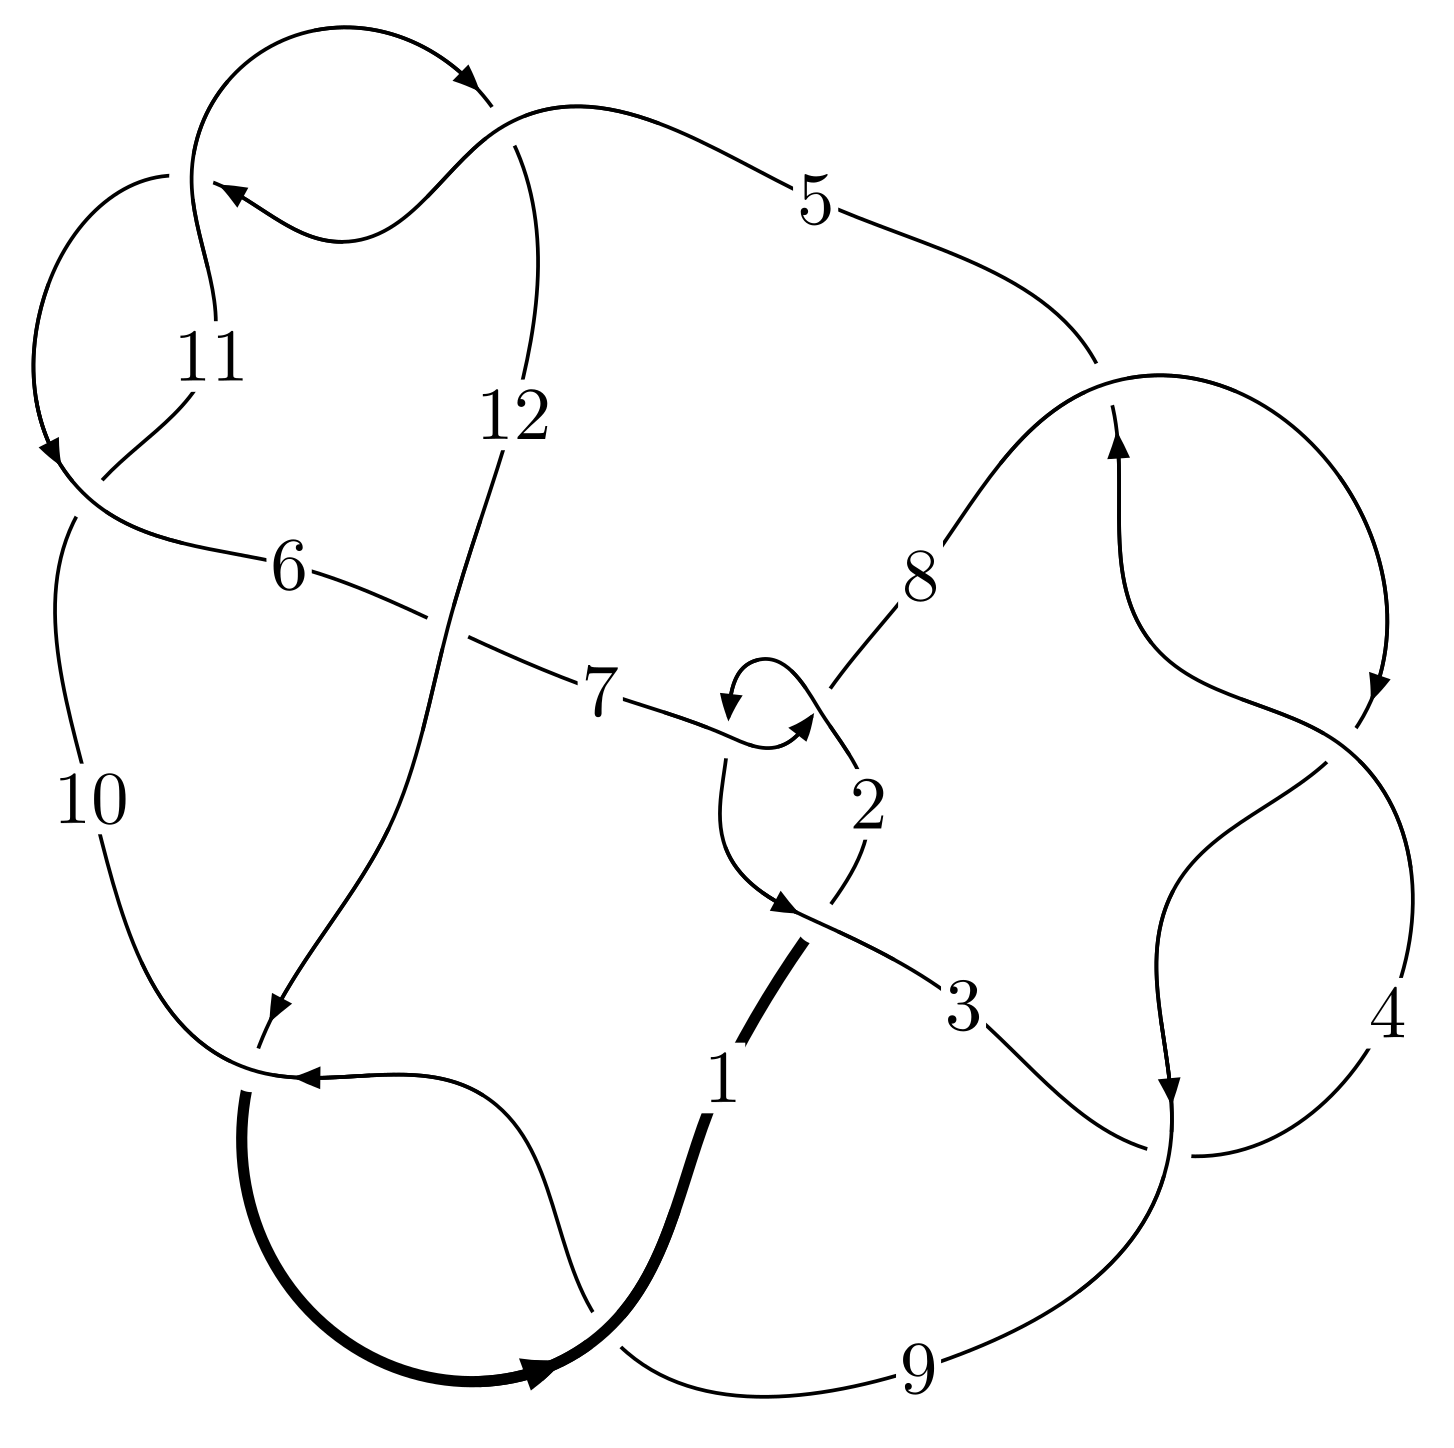
\includegraphics[width=112pt]{../../../GIT/diagram.site/Diagrams/png/1365_12a_0564.png}\\
\ \ \ A knot diagram\footnotemark}&
\allowdisplaybreaks
\textbf{Linearized knot diagam} \\
\cline{2-2}
 &
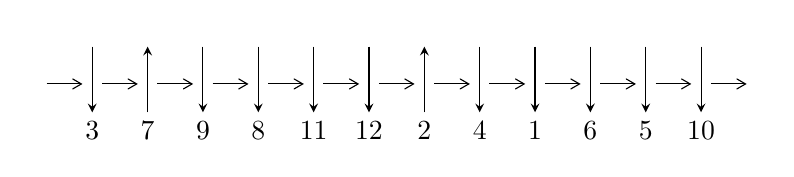
\begin{tikzpicture}[x=20pt, y=17pt]
	% nodes
	\node (C0) at (0, 0) {};
	\node (C1) at (1, 0) {};
	\node (C1U) at (1, +1) {};
	\node (C1D) at (1, -1) {3};

	\node (C2) at (2, 0) {};
	\node (C2U) at (2, +1) {};
	\node (C2D) at (2, -1) {7};

	\node (C3) at (3, 0) {};
	\node (C3U) at (3, +1) {};
	\node (C3D) at (3, -1) {9};

	\node (C4) at (4, 0) {};
	\node (C4U) at (4, +1) {};
	\node (C4D) at (4, -1) {8};

	\node (C5) at (5, 0) {};
	\node (C5U) at (5, +1) {};
	\node (C5D) at (5, -1) {11};

	\node (C6) at (6, 0) {};
	\node (C6U) at (6, +1) {};
	\node (C6D) at (6, -1) {12};

	\node (C7) at (7, 0) {};
	\node (C7U) at (7, +1) {};
	\node (C7D) at (7, -1) {2};

	\node (C8) at (8, 0) {};
	\node (C8U) at (8, +1) {};
	\node (C8D) at (8, -1) {4};

	\node (C9) at (9, 0) {};
	\node (C9U) at (9, +1) {};
	\node (C9D) at (9, -1) {1};

	\node (C10) at (10, 0) {};
	\node (C10U) at (10, +1) {};
	\node (C10D) at (10, -1) {6};

	\node (C11) at (11, 0) {};
	\node (C11U) at (11, +1) {};
	\node (C11D) at (11, -1) {5};

	\node (C12) at (12, 0) {};
	\node (C12U) at (12, +1) {};
	\node (C12D) at (12, -1) {10};
	\node (C13) at (13, 0) {};

	% arrows
	\draw[->,>={angle 60}]
	(C0) edge (C1) (C1) edge (C2) (C2) edge (C3) (C3) edge (C4) (C4) edge (C5) (C5) edge (C6) (C6) edge (C7) (C7) edge (C8) (C8) edge (C9) (C9) edge (C10) (C10) edge (C11) (C11) edge (C12) (C12) edge (C13) ;	\draw[->,>=stealth]
	(C1U) edge (C1D) (C2D) edge (C2U) (C3U) edge (C3D) (C4U) edge (C4D) (C5U) edge (C5D) (C6U) edge (C6D) (C7D) edge (C7U) (C8U) edge (C8D) (C9U) edge (C9D) (C10U) edge (C10D) (C11U) edge (C11D) (C12U) edge (C12D) ;
	\end{tikzpicture} \\
\hhline{~~} \\& 
\textbf{Solving Sequence} \\ \cline{2-2} 
 &
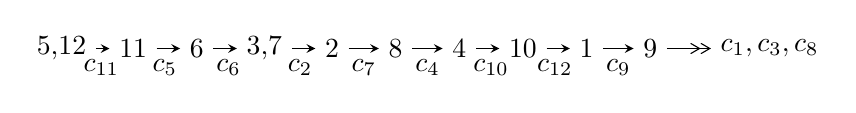
\begin{tikzpicture}[x=23pt, y=7pt]
	% node
	\node (A0) at (-1/8, 0) {5,12};
	\node (A1) at (1, 0) {11};
	\node (A2) at (2, 0) {6};
	\node (A3) at (49/16, 0) {3,7};
	\node (A4) at (33/8, 0) {2};
	\node (A5) at (41/8, 0) {8};
	\node (A6) at (49/8, 0) {4};
	\node (A7) at (57/8, 0) {10};
	\node (A8) at (65/8, 0) {1};
	\node (A9) at (73/8, 0) {9};
	\node (C1) at (1/2, -1) {$c_{11}$};
	\node (C2) at (3/2, -1) {$c_{5}$};
	\node (C3) at (5/2, -1) {$c_{6}$};
	\node (C4) at (29/8, -1) {$c_{2}$};
	\node (C5) at (37/8, -1) {$c_{7}$};
	\node (C6) at (45/8, -1) {$c_{4}$};
	\node (C7) at (53/8, -1) {$c_{10}$};
	\node (C8) at (61/8, -1) {$c_{12}$};
	\node (C9) at (69/8, -1) {$c_{9}$};
	\node (A10) at (11, 0) {$c_{1},c_{3},c_{8}$};

	% edge
	\draw[->,>=stealth]	
	(A0) edge (A1) (A1) edge (A2) (A2) edge (A3) (A3) edge (A4) (A4) edge (A5) (A5) edge (A6) (A6) edge (A7) (A7) edge (A8) (A8) edge (A9) ;
	\draw[->>,>={angle 60}]	
	(A9) edge (A10);
\end{tikzpicture} \\ 

\end{tabular} \\

\footnotetext{
The image of knot diagram is generated by the software ``\textbf{Draw programme}" developed by Andrew Bartholomew(\url{http://www.layer8.co.uk/maths/draw/index.htm\#Running-draw}), where we modified some parts for our purpose(\url{https://github.com/CATsTAILs/LinksPainter}).
}\phantom \\ \newline 
\centering \textbf{Ideals for irreducible components\footnotemark of $X_{\text{par}}$} 
 
\begin{align*}
I^u_{1}&=\langle 
- u^{53}+4 u^{52}+\cdots+4 b+4,\;2 u^{55}-4 u^{54}+\cdots+4 a-12,\;u^{56}-2 u^{55}+\cdots-5 u+2\rangle \\
I^u_{2}&=\langle 
a^2 u^2+2 u^2 a+2 a^2-2 u^2+b+4 a-4,\;2 a^2 u^2+a^3+2 u^2 a+4 a^2+a u-2 u^2+2 a- u-4,\;u^3+2 u-1\rangle \\
I^u_{3}&=\langle 
- u^8+u^7-4 u^6+3 u^5-4 u^4+2 u^3+b- u-1,\;- u^9-5 u^7-8 u^5-3 u^3+a+u,\\
\phantom{I^u_{3}}&\phantom{= \langle  }u^{10}+5 u^8+8 u^6+3 u^4- u^2+1\rangle \\
I^u_{4}&=\langle 
3 a^2 u^2-2 u^3 a+4 a^2 u-2 u^2 a+2 u^3+2 a^2-2 a u+2 u^2+b+2 u,\\
\phantom{I^u_{4}}&\phantom{= \langle  }-2 u^3 a^2-2 a^2 u^2+8 u^3 a+a^3-4 a^2 u+3 u^2 a-2 u^3-4 a^2+13 a u- u^2+8 a-3 u-2,\\
\phantom{I^u_{4}}&\phantom{= \langle  }u^4+u^3+2 u^2+2 u+1\rangle \\
\\
\end{align*}
\raggedright * 4 irreducible components of $\dim_{\mathbb{C}}=0$, with total 87 representations.\\
\footnotetext{All coefficients of polynomials are rational numbers. But the coefficients are sometimes approximated in decimal forms when there is not enough margin.}
\newpage
\renewcommand{\arraystretch}{1}
\centering \section*{I. $I^u_{1}= \langle - u^{53}+4 u^{52}+\cdots+4 b+4,\;2 u^{55}-4 u^{54}+\cdots+4 a-12,\;u^{56}-2 u^{55}+\cdots-5 u+2 \rangle$}
\flushleft \textbf{(i) Arc colorings}\\
\begin{tabular}{m{7pt} m{180pt} m{7pt} m{180pt} }
\flushright $a_{5}=$&$\begin{pmatrix}0\\u\end{pmatrix}$ \\
\flushright $a_{12}=$&$\begin{pmatrix}1\\0\end{pmatrix}$ \\
\flushright $a_{11}=$&$\begin{pmatrix}1\\- u^2\end{pmatrix}$ \\
\flushright $a_{6}=$&$\begin{pmatrix}- u\\u^3+u\end{pmatrix}$ \\
\flushright $a_{3}=$&$\begin{pmatrix}-\frac{1}{2} u^{55}+u^{54}+\cdots-\frac{7}{4} u+3\\\frac{1}{4} u^{53}- u^{52}+\cdots+\frac{3}{2} u-1\end{pmatrix}$ \\
\flushright $a_{7}=$&$\begin{pmatrix}- u^3-2 u\\u^3+u\end{pmatrix}$ \\
\flushright $a_{2}=$&$\begin{pmatrix}\frac{1}{4} u^{51}+6 u^{49}+\cdots+\frac{5}{4} u+1\\-\frac{1}{4} u^{53}-\frac{25}{4} u^{51}+\cdots+\frac{1}{2} u^2+\frac{1}{2} u\end{pmatrix}$ \\
\flushright $a_{8}=$&$\begin{pmatrix}-\frac{1}{4} u^{55}-\frac{13}{2} u^{53}+\cdots-\frac{1}{4} u-1\\\frac{3}{4} u^{55}- u^{54}+\cdots+\frac{5}{2} u-1\end{pmatrix}$ \\
\flushright $a_{4}=$&$\begin{pmatrix}\frac{1}{4} u^{44}+\frac{21}{4} u^{42}+\cdots+\frac{1}{2} u+\frac{1}{2}\\-\frac{1}{4} u^{44}-5 u^{42}+\cdots-\frac{3}{4} u^2+u\end{pmatrix}$ \\
\flushright $a_{10}=$&$\begin{pmatrix}u^2+1\\- u^4-2 u^2\end{pmatrix}$ \\
\flushright $a_{1}=$&$\begin{pmatrix}- u^6-3 u^4-2 u^2+1\\u^8+4 u^6+4 u^4\end{pmatrix}$ \\
\flushright $a_{9}=$&$\begin{pmatrix}u^{10}+5 u^8+8 u^6+3 u^4- u^2+1\\- u^{12}-6 u^{10}-12 u^8-8 u^6- u^4-2 u^2\end{pmatrix}$\\&\end{tabular}
\flushleft \textbf{(ii) Obstruction class $= -1$}\\~\\
\flushleft \textbf{(iii) Cusp Shapes $= 2 u^{55}-4 u^{54}+\cdots+20 u-10$}\\~\\
\newpage\renewcommand{\arraystretch}{1}
\flushleft \textbf{(iv) u-Polynomials at the component}\newline \\
\begin{tabular}{m{50pt}|m{274pt}}
Crossings & \hspace{64pt}u-Polynomials at each crossing \\
\hline $$\begin{aligned}c_{1}\end{aligned}$$&$\begin{aligned}
&u^{56}+19 u^{55}+\cdots-20 u+1
\end{aligned}$\\
\hline $$\begin{aligned}c_{2},c_{7}\end{aligned}$$&$\begin{aligned}
&u^{56}+u^{55}+\cdots-10 u^2+1
\end{aligned}$\\
\hline $$\begin{aligned}c_{3},c_{4},c_{8}\end{aligned}$$&$\begin{aligned}
&u^{56}+u^{55}+\cdots+2 u+1
\end{aligned}$\\
\hline $$\begin{aligned}c_{5},c_{10},c_{11}\end{aligned}$$&$\begin{aligned}
&u^{56}+2 u^{55}+\cdots+5 u+2
\end{aligned}$\\
\hline $$\begin{aligned}c_{6}\end{aligned}$$&$\begin{aligned}
&u^{56}-2 u^{55}+\cdots-231 u+202
\end{aligned}$\\
\hline $$\begin{aligned}c_{9},c_{12}\end{aligned}$$&$\begin{aligned}
&u^{56}-8 u^{55}+\cdots-1317 u+136
\end{aligned}$\\
\hline
\end{tabular}\\~\\
\newpage\renewcommand{\arraystretch}{1}
\flushleft \textbf{(v) Riley Polynomials at the component}\newline \\
\begin{tabular}{m{50pt}|m{274pt}}
Crossings & \hspace{64pt}Riley Polynomials at each crossing \\
\hline $$\begin{aligned}c_{1}\end{aligned}$$&$\begin{aligned}
&y^{56}+47 y^{55}+\cdots+1224 y+1
\end{aligned}$\\
\hline $$\begin{aligned}c_{2},c_{7}\end{aligned}$$&$\begin{aligned}
&y^{56}+19 y^{55}+\cdots-20 y+1
\end{aligned}$\\
\hline $$\begin{aligned}c_{3},c_{4},c_{8}\end{aligned}$$&$\begin{aligned}
&y^{56}+63 y^{55}+\cdots-84 y+1
\end{aligned}$\\
\hline $$\begin{aligned}c_{5},c_{10},c_{11}\end{aligned}$$&$\begin{aligned}
&y^{56}+52 y^{55}+\cdots+19 y+4
\end{aligned}$\\
\hline $$\begin{aligned}c_{6}\end{aligned}$$&$\begin{aligned}
&y^{56}+20 y^{55}+\cdots+498907 y+40804
\end{aligned}$\\
\hline $$\begin{aligned}c_{9},c_{12}\end{aligned}$$&$\begin{aligned}
&y^{56}+48 y^{55}+\cdots-423177 y+18496
\end{aligned}$\\
\hline
\end{tabular}\\~\\
\newpage\flushleft \textbf{(vi) Complex Volumes and Cusp Shapes}
$$\begin{array}{c|c|c}  
\text{Solutions to }I^u_{1}& \I (\text{vol} + \sqrt{-1}CS) & \text{Cusp shape}\\
 \hline 
\begin{aligned}
u &= \phantom{-}0.167031 + 1.023460 I \\
a &= \phantom{-}0.581239 + 0.389226 I \\
b &= \phantom{-}0.786716 - 0.931788 I\end{aligned}
 & \phantom{-}4.78319 + 2.48153 I & -3.50379 - 2.32484 I \\ \hline\begin{aligned}
u &= \phantom{-}0.167031 - 1.023460 I \\
a &= \phantom{-}0.581239 - 0.389226 I \\
b &= \phantom{-}0.786716 + 0.931788 I\end{aligned}
 & \phantom{-}4.78319 - 2.48153 I & -3.50379 + 2.32484 I \\ \hline\begin{aligned}
u &= \phantom{-}0.692071 + 0.437803 I \\
a &= -0.66383 - 2.04682 I \\
b &= -0.37969 + 1.48563 I\end{aligned}
 & \phantom{-}10.54030 - 5.20317 I & -1.76462 + 3.90235 I \\ \hline\begin{aligned}
u &= \phantom{-}0.692071 - 0.437803 I \\
a &= -0.66383 + 2.04682 I \\
b &= -0.37969 - 1.48563 I\end{aligned}
 & \phantom{-}10.54030 + 5.20317 I & -1.76462 - 3.90235 I \\ \hline\begin{aligned}
u &= -0.708508 + 0.410403 I \\
a &= \phantom{-}1.96906 - 2.08951 I \\
b &= -1.10648 + 2.12776 I\end{aligned}
 & \phantom{-}8.5419 + 11.5420 I & -4.16165 - 8.13234 I \\ \hline\begin{aligned}
u &= -0.708508 - 0.410403 I \\
a &= \phantom{-}1.96906 + 2.08951 I \\
b &= -1.10648 - 2.12776 I\end{aligned}
 & \phantom{-}8.5419 - 11.5420 I & -4.16165 + 8.13234 I \\ \hline\begin{aligned}
u &= \phantom{-}0.622613 + 0.525563 I \\
a &= \phantom{-}1.77821 + 0.87570 I \\
b &= -0.85453 - 1.37150 I\end{aligned}
 & \phantom{-}10.86790 + 0.81891 I & -1.02610 + 2.14303 I \\ \hline\begin{aligned}
u &= \phantom{-}0.622613 - 0.525563 I \\
a &= \phantom{-}1.77821 - 0.87570 I \\
b &= -0.85453 + 1.37150 I\end{aligned}
 & \phantom{-}10.86790 - 0.81891 I & -1.02610 - 2.14303 I \\ \hline\begin{aligned}
u &= -0.592033 + 0.557273 I \\
a &= -1.57209 + 2.23463 I \\
b &= -0.22451 - 1.53219 I\end{aligned}
 & \phantom{-}9.08740 - 7.17759 I & -2.84487 + 2.35339 I \\ \hline\begin{aligned}
u &= -0.592033 - 0.557273 I \\
a &= -1.57209 - 2.23463 I \\
b &= -0.22451 + 1.53219 I\end{aligned}
 & \phantom{-}9.08740 + 7.17759 I & -2.84487 - 2.35339 I\\
 \hline 
 \end{array}$$\newpage$$\begin{array}{c|c|c}  
\text{Solutions to }I^u_{1}& \I (\text{vol} + \sqrt{-1}CS) & \text{Cusp shape}\\
 \hline 
\begin{aligned}
u &= -0.103142 + 1.185330 I \\
a &= \phantom{-}0.186061 - 0.410343 I \\
b &= \phantom{-}1.46690 + 0.65983 I\end{aligned}
 & -0.051945 - 0.385761 I & \phantom{-0.000000 } 0 \\ \hline\begin{aligned}
u &= -0.103142 - 1.185330 I \\
a &= \phantom{-}0.186061 + 0.410343 I \\
b &= \phantom{-}1.46690 - 0.65983 I\end{aligned}
 & -0.051945 + 0.385761 I & \phantom{-0.000000 } 0 \\ \hline\begin{aligned}
u &= \phantom{-}0.669252 + 0.412330 I \\
a &= \phantom{-}2.47043 + 1.87049 I \\
b &= -1.39269 - 1.97696 I\end{aligned}
 & \phantom{-}2.26755 - 7.24573 I & -6.66677 + 8.30952 I \\ \hline\begin{aligned}
u &= \phantom{-}0.669252 - 0.412330 I \\
a &= \phantom{-}2.47043 - 1.87049 I \\
b &= -1.39269 + 1.97696 I\end{aligned}
 & \phantom{-}2.26755 + 7.24573 I & -6.66677 - 8.30952 I \\ \hline\begin{aligned}
u &= -0.206699 + 0.752355 I \\
a &= \phantom{-}0.574163 - 0.045388 I \\
b &= \phantom{-}0.468649 - 0.514420 I\end{aligned}
 & \phantom{-}4.95627 + 2.53829 I & -2.18457 - 3.78654 I \\ \hline\begin{aligned}
u &= -0.206699 - 0.752355 I \\
a &= \phantom{-}0.574163 + 0.045388 I \\
b &= \phantom{-}0.468649 + 0.514420 I\end{aligned}
 & \phantom{-}4.95627 - 2.53829 I & -2.18457 + 3.78654 I \\ \hline\begin{aligned}
u &= \phantom{-}0.582613 + 0.498044 I \\
a &= -1.36009 - 2.66583 I \\
b &= -0.26540 + 1.65618 I\end{aligned}
 & \phantom{-}2.62946 + 3.09884 I & -5.44089 - 2.20028 I \\ \hline\begin{aligned}
u &= \phantom{-}0.582613 - 0.498044 I \\
a &= -1.36009 + 2.66583 I \\
b &= -0.26540 - 1.65618 I\end{aligned}
 & \phantom{-}2.62946 - 3.09884 I & -5.44089 + 2.20028 I \\ \hline\begin{aligned}
u &= -0.676046 + 0.203719 I \\
a &= \phantom{-}0.329443 + 0.139721 I \\
b &= \phantom{-}0.294607 - 0.292968 I\end{aligned}
 & \phantom{-}3.00074 + 0.91231 I & -5.60324 - 1.33604 I \\ \hline\begin{aligned}
u &= -0.676046 - 0.203719 I \\
a &= \phantom{-}0.329443 - 0.139721 I \\
b &= \phantom{-}0.294607 + 0.292968 I\end{aligned}
 & \phantom{-}3.00074 - 0.91231 I & -5.60324 + 1.33604 I\\
 \hline 
 \end{array}$$\newpage$$\begin{array}{c|c|c}  
\text{Solutions to }I^u_{1}& \I (\text{vol} + \sqrt{-1}CS) & \text{Cusp shape}\\
 \hline 
\begin{aligned}
u &= \phantom{-}0.692318 + 0.121292 I \\
a &= -0.85392 - 1.33610 I \\
b &= \phantom{-}0.25519 + 1.45796 I\end{aligned}
 & \phantom{-}2.08625 - 5.88981 I & -8.03014 + 6.36741 I \\ \hline\begin{aligned}
u &= \phantom{-}0.692318 - 0.121292 I \\
a &= -0.85392 + 1.33610 I \\
b &= \phantom{-}0.25519 - 1.45796 I\end{aligned}
 & \phantom{-}2.08625 + 5.88981 I & -8.03014 - 6.36741 I \\ \hline\begin{aligned}
u &= -0.201418 + 1.293670 I \\
a &= -0.870058 - 0.579976 I \\
b &= -0.43169 - 1.56082 I\end{aligned}
 & \phantom{-}1.14651 + 5.97963 I & \phantom{-0.000000 } 0 \\ \hline\begin{aligned}
u &= -0.201418 - 1.293670 I \\
a &= -0.870058 + 0.579976 I \\
b &= -0.43169 + 1.56082 I\end{aligned}
 & \phantom{-}1.14651 - 5.97963 I & \phantom{-0.000000 } 0 \\ \hline\begin{aligned}
u &= \phantom{-}0.261428 + 1.299180 I \\
a &= -1.039600 + 0.218945 I \\
b &= -0.49696 + 1.44809 I\end{aligned}
 & \phantom{-}6.50957 - 9.34599 I & \phantom{-0.000000 } 0 \\ \hline\begin{aligned}
u &= \phantom{-}0.261428 - 1.299180 I \\
a &= -1.039600 - 0.218945 I \\
b &= -0.49696 - 1.44809 I\end{aligned}
 & \phantom{-}6.50957 + 9.34599 I & \phantom{-0.000000 } 0 \\ \hline\begin{aligned}
u &= \phantom{-}0.580660 + 0.311133 I \\
a &= \phantom{-}0.0703685 - 0.0523659 I \\
b &= \phantom{-}0.409701 + 0.523982 I\end{aligned}
 & -1.38214 - 1.50697 I & -13.53047 + 3.87884 I \\ \hline\begin{aligned}
u &= \phantom{-}0.580660 - 0.311133 I \\
a &= \phantom{-}0.0703685 + 0.0523659 I \\
b &= \phantom{-}0.409701 - 0.523982 I\end{aligned}
 & -1.38214 + 1.50697 I & -13.53047 - 3.87884 I \\ \hline\begin{aligned}
u &= -0.008074 + 1.347070 I \\
a &= \phantom{-}0.668271 + 0.576392 I \\
b &= \phantom{-}0.353028 + 0.821443 I\end{aligned}
 & \phantom{-}4.43635 - 1.45929 I & \phantom{-0.000000 } 0 \\ \hline\begin{aligned}
u &= -0.008074 - 1.347070 I \\
a &= \phantom{-}0.668271 - 0.576392 I \\
b &= \phantom{-}0.353028 - 0.821443 I\end{aligned}
 & \phantom{-}4.43635 + 1.45929 I & \phantom{-0.000000 } 0\\
 \hline 
 \end{array}$$\newpage$$\begin{array}{c|c|c}  
\text{Solutions to }I^u_{1}& \I (\text{vol} + \sqrt{-1}CS) & \text{Cusp shape}\\
 \hline 
\begin{aligned}
u &= -0.521433 + 0.341179 I \\
a &= \phantom{-}1.33055 + 0.94373 I \\
b &= -0.774976 - 0.280233 I\end{aligned}
 & \phantom{-}2.02037 + 1.59760 I & -0.90500 - 4.85866 I \\ \hline\begin{aligned}
u &= -0.521433 - 0.341179 I \\
a &= \phantom{-}1.33055 - 0.94373 I \\
b &= -0.774976 + 0.280233 I\end{aligned}
 & \phantom{-}2.02037 - 1.59760 I & -0.90500 + 4.85866 I \\ \hline\begin{aligned}
u &= -0.246474 + 1.358800 I \\
a &= \phantom{-}0.252006 + 0.237582 I \\
b &= -0.157937 - 0.612956 I\end{aligned}
 & \phantom{-}7.93137 + 4.24929 I & \phantom{-0.000000 } 0 \\ \hline\begin{aligned}
u &= -0.246474 - 1.358800 I \\
a &= \phantom{-}0.252006 - 0.237582 I \\
b &= -0.157937 + 0.612956 I\end{aligned}
 & \phantom{-}7.93137 - 4.24929 I & \phantom{-0.000000 } 0 \\ \hline\begin{aligned}
u &= -0.604464 + 0.090171 I \\
a &= -1.22485 + 0.96150 I \\
b &= \phantom{-}0.55744 - 1.31425 I\end{aligned}
 & -3.13696 + 3.05067 I & -15.3053 - 6.1769 I \\ \hline\begin{aligned}
u &= -0.604464 - 0.090171 I \\
a &= -1.22485 - 0.96150 I \\
b &= \phantom{-}0.55744 + 1.31425 I\end{aligned}
 & -3.13696 - 3.05067 I & -15.3053 + 6.1769 I \\ \hline\begin{aligned}
u &= -0.20414 + 1.41040 I \\
a &= \phantom{-}0.154106 + 0.721195 I \\
b &= -1.068550 - 0.531298 I\end{aligned}
 & \phantom{-}7.58921 + 4.29042 I & \phantom{-0.000000 } 0 \\ \hline\begin{aligned}
u &= -0.20414 - 1.41040 I \\
a &= \phantom{-}0.154106 - 0.721195 I \\
b &= -1.068550 + 0.531298 I\end{aligned}
 & \phantom{-}7.58921 - 4.29042 I & \phantom{-0.000000 } 0 \\ \hline\begin{aligned}
u &= \phantom{-}0.22437 + 1.42514 I \\
a &= \phantom{-}0.0464407 - 0.0037704 I \\
b &= -0.198621 + 1.070760 I\end{aligned}
 & \phantom{-}4.20552 - 4.47801 I & \phantom{-0.000000 } 0 \\ \hline\begin{aligned}
u &= \phantom{-}0.22437 - 1.42514 I \\
a &= \phantom{-}0.0464407 + 0.0037704 I \\
b &= -0.198621 - 1.070760 I\end{aligned}
 & \phantom{-}4.20552 + 4.47801 I & \phantom{-0.000000 } 0\\
 \hline 
 \end{array}$$\newpage$$\begin{array}{c|c|c}  
\text{Solutions to }I^u_{1}& \I (\text{vol} + \sqrt{-1}CS) & \text{Cusp shape}\\
 \hline 
\begin{aligned}
u &= -0.02481 + 1.45160 I \\
a &= \phantom{-}0.437034 - 0.432649 I \\
b &= -0.071252 - 1.121650 I\end{aligned}
 & \phantom{-}11.67150 + 3.02727 I & \phantom{-0.000000 } 0 \\ \hline\begin{aligned}
u &= -0.02481 - 1.45160 I \\
a &= \phantom{-}0.437034 + 0.432649 I \\
b &= -0.071252 + 1.121650 I\end{aligned}
 & \phantom{-}11.67150 - 3.02727 I & \phantom{-0.000000 } 0 \\ \hline\begin{aligned}
u &= \phantom{-}0.24729 + 1.46542 I \\
a &= \phantom{-}1.75227 - 0.41488 I \\
b &= -1.92961 - 2.80986 I\end{aligned}
 & \phantom{-}8.32154 - 10.59610 I & \phantom{-0.000000 } 0 \\ \hline\begin{aligned}
u &= \phantom{-}0.24729 - 1.46542 I \\
a &= \phantom{-}1.75227 + 0.41488 I \\
b &= -1.92961 + 2.80986 I\end{aligned}
 & \phantom{-}8.32154 + 10.59610 I & \phantom{-0.000000 } 0 \\ \hline\begin{aligned}
u &= \phantom{-}0.20280 + 1.47543 I \\
a &= -1.64369 - 0.44402 I \\
b &= \phantom{-}0.68333 + 2.27056 I\end{aligned}
 & \phantom{-}8.98647 + 0.24581 I & \phantom{-0.000000 } 0 \\ \hline\begin{aligned}
u &= \phantom{-}0.20280 - 1.47543 I \\
a &= -1.64369 + 0.44402 I \\
b &= \phantom{-}0.68333 - 2.27056 I\end{aligned}
 & \phantom{-}8.98647 - 0.24581 I & \phantom{-0.000000 } 0 \\ \hline\begin{aligned}
u &= -0.26313 + 1.47028 I \\
a &= \phantom{-}1.68249 + 0.12616 I \\
b &= -1.40694 + 2.97582 I\end{aligned}
 & \phantom{-}14.6067 + 15.0877 I & \phantom{-0.000000 } 0 \\ \hline\begin{aligned}
u &= -0.26313 - 1.47028 I \\
a &= \phantom{-}1.68249 - 0.12616 I \\
b &= -1.40694 - 2.97582 I\end{aligned}
 & \phantom{-}14.6067 - 15.0877 I & \phantom{-0.000000 } 0 \\ \hline\begin{aligned}
u &= \phantom{-}0.25179 + 1.47848 I \\
a &= -1.236920 - 0.501404 I \\
b &= -0.07447 + 1.78181 I\end{aligned}
 & \phantom{-}16.7327 - 8.6480 I & \phantom{-0.000000 } 0 \\ \hline\begin{aligned}
u &= \phantom{-}0.25179 - 1.47848 I \\
a &= -1.236920 + 0.501404 I \\
b &= -0.07447 - 1.78181 I\end{aligned}
 & \phantom{-}16.7327 + 8.6480 I & \phantom{-0.000000 } 0\\
 \hline 
 \end{array}$$\newpage$$\begin{array}{c|c|c}  
\text{Solutions to }I^u_{1}& \I (\text{vol} + \sqrt{-1}CS) & \text{Cusp shape}\\
 \hline 
\begin{aligned}
u &= -0.18754 + 1.49529 I \\
a &= -1.54445 + 0.24504 I \\
b &= \phantom{-}0.90159 - 1.78028 I\end{aligned}
 & \phantom{-}15.7506 - 4.3922 I & \phantom{-0.000000 } 0 \\ \hline\begin{aligned}
u &= -0.18754 - 1.49529 I \\
a &= -1.54445 - 0.24504 I \\
b &= \phantom{-}0.90159 + 1.78028 I\end{aligned}
 & \phantom{-}15.7506 + 4.3922 I & \phantom{-0.000000 } 0 \\ \hline\begin{aligned}
u &= \phantom{-}0.20634 + 1.49448 I \\
a &= \phantom{-}1.075950 - 0.501942 I \\
b &= -1.36447 - 1.63496 I\end{aligned}
 & \phantom{-}17.4257 - 2.1759 I & \phantom{-0.000000 } 0 \\ \hline\begin{aligned}
u &= \phantom{-}0.20634 - 1.49448 I \\
a &= \phantom{-}1.075950 + 0.501942 I \\
b &= -1.36447 + 1.63496 I\end{aligned}
 & \phantom{-}17.4257 + 2.1759 I & \phantom{-0.000000 } 0 \\ \hline\begin{aligned}
u &= \phantom{-}0.147340 + 0.378273 I \\
a &= \phantom{-}0.901441 + 0.594340 I \\
b &= \phantom{-}0.521618 + 0.321445 I\end{aligned}
 & -0.581405 - 1.167200 I & -7.43245 + 5.35431 I \\ \hline\begin{aligned}
u &= \phantom{-}0.147340 - 0.378273 I \\
a &= \phantom{-}0.901441 - 0.594340 I \\
b &= \phantom{-}0.521618 - 0.321445 I\end{aligned}
 & -0.581405 + 1.167200 I & -7.43245 - 5.35431 I\\
 \hline 
 \end{array}$$\newpage\newpage\renewcommand{\arraystretch}{1}
\centering \section*{II. $I^u_{2}= \langle a^2 u^2+2 u^2 a+2 a^2-2 u^2+b+4 a-4,\;2 a^2 u^2+2 u^2 a+\cdots+2 a-4,\;u^3+2 u-1 \rangle$}
\flushleft \textbf{(i) Arc colorings}\\
\begin{tabular}{m{7pt} m{180pt} m{7pt} m{180pt} }
\flushright $a_{5}=$&$\begin{pmatrix}0\\u\end{pmatrix}$ \\
\flushright $a_{12}=$&$\begin{pmatrix}1\\0\end{pmatrix}$ \\
\flushright $a_{11}=$&$\begin{pmatrix}1\\- u^2\end{pmatrix}$ \\
\flushright $a_{6}=$&$\begin{pmatrix}- u\\- u+1\end{pmatrix}$ \\
\flushright $a_{3}=$&$\begin{pmatrix}a\\- a^2 u^2-2 u^2 a-2 a^2+2 u^2-4 a+4\end{pmatrix}$ \\
\flushright $a_{7}=$&$\begin{pmatrix}-1\\- u+1\end{pmatrix}$ \\
\flushright $a_{2}=$&$\begin{pmatrix}a^2 u^2+2 u^2 a+2 a^2+a u-2 u^2+4 a-4\\-2 a^2 u^2-3 u^2 a-3 a^2-2 a u+4 u^2-5 a+6\end{pmatrix}$ \\
\flushright $a_{8}=$&$\begin{pmatrix}2 a^2 u^2+a^2 u+3 u^2 a+4 a^2+2 a u-4 u^2+7 a-2 u-8\\- a^2 u^2- a^2 u- a^2- a u+2 u^2-2 a+2 u+2\end{pmatrix}$ \\
\flushright $a_{4}=$&$\begin{pmatrix}a^2 u^2+2 u^2 a+2 a^2+a u-2 u^2+4 a-4\\-2 a^2 u^2-3 u^2 a-3 a^2-2 a u+4 u^2-5 a+6\end{pmatrix}$ \\
\flushright $a_{10}=$&$\begin{pmatrix}u^2+1\\- u\end{pmatrix}$ \\
\flushright $a_{1}=$&$\begin{pmatrix}u\\u^2\end{pmatrix}$ \\
\flushright $a_{9}=$&$\begin{pmatrix}1\\u-1\end{pmatrix}$\\&\end{tabular}
\flushleft \textbf{(ii) Obstruction class $= -1$}\\~\\
\flushleft \textbf{(iii) Cusp Shapes $= -4 u^2-4 u-10$}\\~\\
\newpage\renewcommand{\arraystretch}{1}
\flushleft \textbf{(iv) u-Polynomials at the component}\newline \\
\begin{tabular}{m{50pt}|m{274pt}}
Crossings & \hspace{64pt}u-Polynomials at each crossing \\
\hline $$\begin{aligned}c_{1}\end{aligned}$$&$\begin{aligned}
&u^9+6 u^8+15 u^7+24 u^6+31 u^5+30 u^4+21 u^3+12 u^2+4 u-1
\end{aligned}$\\
\hline $$\begin{aligned}c_{2},c_{3},c_{4}\\c_{7},c_{8}\end{aligned}$$&$\begin{aligned}
&u^9+3 u^7+3 u^5+3 u^3+2 u+1
\end{aligned}$\\
\hline $$\begin{aligned}c_{5},c_{9},c_{10}\\c_{11},c_{12}\end{aligned}$$&$\begin{aligned}
&(u^3+2 u+1)^3
\end{aligned}$\\
\hline $$\begin{aligned}c_{6}\end{aligned}$$&$\begin{aligned}
&(u^3+3 u^2+5 u+2)^3
\end{aligned}$\\
\hline
\end{tabular}\\~\\
\newpage\renewcommand{\arraystretch}{1}
\flushleft \textbf{(v) Riley Polynomials at the component}\newline \\
\begin{tabular}{m{50pt}|m{274pt}}
Crossings & \hspace{64pt}Riley Polynomials at each crossing \\
\hline $$\begin{aligned}c_{1}\end{aligned}$$&$\begin{aligned}
&y^9-6 y^8- y^7+36 y^6+15 y^5-42 y^4+17 y^3+84 y^2+40 y-1
\end{aligned}$\\
\hline $$\begin{aligned}c_{2},c_{3},c_{4}\\c_{7},c_{8}\end{aligned}$$&$\begin{aligned}
&y^9+6 y^8+15 y^7+24 y^6+31 y^5+30 y^4+21 y^3+12 y^2+4 y-1
\end{aligned}$\\
\hline $$\begin{aligned}c_{5},c_{9},c_{10}\\c_{11},c_{12}\end{aligned}$$&$\begin{aligned}
&(y^3+4 y^2+4 y-1)^3
\end{aligned}$\\
\hline $$\begin{aligned}c_{6}\end{aligned}$$&$\begin{aligned}
&(y^3+y^2+13 y-4)^3
\end{aligned}$\\
\hline
\end{tabular}\\~\\
\newpage\flushleft \textbf{(vi) Complex Volumes and Cusp Shapes}
$$\begin{array}{c|c|c}  
\text{Solutions to }I^u_{2}& \I (\text{vol} + \sqrt{-1}CS) & \text{Cusp shape}\\
 \hline 
\begin{aligned}
u &= -0.22670 + 1.46771 I \\
a &= -1.41033 + 0.65322 I \\
b &= \phantom{-}0.02182 - 2.22338 I\end{aligned}
 & \phantom{-}9.44074 + 5.13794 I & -0.68207 - 3.20902 I \\ \hline\begin{aligned}
u &= -0.22670 + 1.46771 I \\
a &= \phantom{-}1.44687 + 0.73836 I \\
b &= -2.15352 + 1.99644 I\end{aligned}
 & \phantom{-}9.44074 + 5.13794 I & -0.68207 - 3.20902 I \\ \hline\begin{aligned}
u &= -0.22670 + 1.46771 I \\
a &= \phantom{-}0.169027 - 0.060668 I \\
b &= -0.073872 - 1.103970 I\end{aligned}
 & \phantom{-}9.44074 + 5.13794 I & -0.68207 - 3.20902 I \\ \hline\begin{aligned}
u &= -0.22670 - 1.46771 I \\
a &= -1.41033 - 0.65322 I \\
b &= \phantom{-}0.02182 + 2.22338 I\end{aligned}
 & \phantom{-}9.44074 - 5.13794 I & -0.68207 + 3.20902 I \\ \hline\begin{aligned}
u &= -0.22670 - 1.46771 I \\
a &= \phantom{-}1.44687 - 0.73836 I \\
b &= -2.15352 - 1.99644 I\end{aligned}
 & \phantom{-}9.44074 - 5.13794 I & -0.68207 + 3.20902 I \\ \hline\begin{aligned}
u &= -0.22670 - 1.46771 I \\
a &= \phantom{-}0.169027 + 0.060668 I \\
b &= -0.073872 + 1.103970 I\end{aligned}
 & \phantom{-}9.44074 - 5.13794 I & -0.68207 + 3.20902 I \\ \hline\begin{aligned}
u &= \phantom{-}0.453398\phantom{ +0.000000I} \\
a &= \phantom{-}0.733086\phantom{ +0.000000I} \\
b &= -0.00791217\phantom{ +0.000000I}\end{aligned}
 & -0.787199\phantom{ +0.000000I} & -12.6360\phantom{ +0.000000I} \\ \hline\begin{aligned}
u &= \phantom{-}0.453398\phantom{ +0.000000I} \\
a &= -2.57211 + 0.14119 I \\
b &= \phantom{-}1.20953 + 0.97910 I\end{aligned}
 & -0.787199\phantom{ +0.000000I} & -12.6360\phantom{ +0.000000I} \\ \hline\begin{aligned}
u &= \phantom{-}0.453398\phantom{ +0.000000I} \\
a &= -2.57211 - 0.14119 I \\
b &= \phantom{-}1.20953 - 0.97910 I\end{aligned}
 & -0.787199\phantom{ +0.000000I} & -12.6360\phantom{ +0.000000I}\\
 \hline 
 \end{array}$$\newpage\newpage\renewcommand{\arraystretch}{1}
\centering \section*{III. $I^u_{3}= \langle - u^8+u^7-4 u^6+3 u^5-4 u^4+2 u^3+b- u-1,\;- u^9-5 u^7-8 u^5-3 u^3+a+u,\;u^{10}+5 u^8+8 u^6+3 u^4- u^2+1 \rangle$}
\flushleft \textbf{(i) Arc colorings}\\
\begin{tabular}{m{7pt} m{180pt} m{7pt} m{180pt} }
\flushright $a_{5}=$&$\begin{pmatrix}0\\u\end{pmatrix}$ \\
\flushright $a_{12}=$&$\begin{pmatrix}1\\0\end{pmatrix}$ \\
\flushright $a_{11}=$&$\begin{pmatrix}1\\- u^2\end{pmatrix}$ \\
\flushright $a_{6}=$&$\begin{pmatrix}- u\\u^3+u\end{pmatrix}$ \\
\flushright $a_{3}=$&$\begin{pmatrix}u^9+5 u^7+8 u^5+3 u^3- u\\u^8- u^7+4 u^6-3 u^5+4 u^4-2 u^3+u+1\end{pmatrix}$ \\
\flushright $a_{7}=$&$\begin{pmatrix}- u^3-2 u\\u^3+u\end{pmatrix}$ \\
\flushright $a_{2}=$&$\begin{pmatrix}u^9+5 u^7- u^6+8 u^5-3 u^4+3 u^3-2 u^2- u+1\\2 u^8- u^7+8 u^6-3 u^5+8 u^4-2 u^3+u+1\end{pmatrix}$ \\
\flushright $a_{8}=$&$\begin{pmatrix}- u^8-4 u^6-5 u^4-2 u^2-1\\u^9+4 u^7+5 u^5+u^4+u^3+2 u^2\end{pmatrix}$ \\
\flushright $a_{4}=$&$\begin{pmatrix}u^9+5 u^7+8 u^5+3 u^3- u\\u^8- u^7+4 u^6-3 u^5+4 u^4-2 u^3+2 u+1\end{pmatrix}$ \\
\flushright $a_{10}=$&$\begin{pmatrix}u^2+1\\- u^4-2 u^2\end{pmatrix}$ \\
\flushright $a_{1}=$&$\begin{pmatrix}- u^6-3 u^4-2 u^2+1\\u^8+4 u^6+4 u^4\end{pmatrix}$ \\
\flushright $a_{9}=$&$\begin{pmatrix}0\\u^8+3 u^6+u^4-2 u^2+1\end{pmatrix}$\\&\end{tabular}
\flushleft \textbf{(ii) Obstruction class $= 1$}\\~\\
\flushleft \textbf{(iii) Cusp Shapes $= 4 u^6+12 u^4+8 u^2-8$}\\~\\
\newpage\renewcommand{\arraystretch}{1}
\flushleft \textbf{(iv) u-Polynomials at the component}\newline \\
\begin{tabular}{m{50pt}|m{274pt}}
Crossings & \hspace{64pt}u-Polynomials at each crossing \\
\hline $$\begin{aligned}c_{1}\end{aligned}$$&$\begin{aligned}
&(u-1)^{10}
\end{aligned}$\\
\hline $$\begin{aligned}c_{2},c_{3},c_{4}\\c_{7},c_{8}\end{aligned}$$&$\begin{aligned}
&(u^2+1)^5
\end{aligned}$\\
\hline $$\begin{aligned}c_{5},c_{10},c_{11}\end{aligned}$$&$\begin{aligned}
&u^{10}+5 u^8+8 u^6+3 u^4- u^2+1
\end{aligned}$\\
\hline $$\begin{aligned}c_{6}\end{aligned}$$&$\begin{aligned}
&u^{10}+u^8+8 u^6+3 u^4+3 u^2+1
\end{aligned}$\\
\hline $$\begin{aligned}c_{9}\end{aligned}$$&$\begin{aligned}
&(u^5+u^4+2 u^3+u^2+u+1)^2
\end{aligned}$\\
\hline $$\begin{aligned}c_{12}\end{aligned}$$&$\begin{aligned}
&(u^5- u^4+2 u^3- u^2+u-1)^2
\end{aligned}$\\
\hline
\end{tabular}\\~\\
\newpage\renewcommand{\arraystretch}{1}
\flushleft \textbf{(v) Riley Polynomials at the component}\newline \\
\begin{tabular}{m{50pt}|m{274pt}}
Crossings & \hspace{64pt}Riley Polynomials at each crossing \\
\hline $$\begin{aligned}c_{1}\end{aligned}$$&$\begin{aligned}
&(y-1)^{10}
\end{aligned}$\\
\hline $$\begin{aligned}c_{2},c_{3},c_{4}\\c_{7},c_{8}\end{aligned}$$&$\begin{aligned}
&(y+1)^{10}
\end{aligned}$\\
\hline $$\begin{aligned}c_{5},c_{10},c_{11}\end{aligned}$$&$\begin{aligned}
&(y^5+5 y^4+8 y^3+3 y^2- y+1)^2
\end{aligned}$\\
\hline $$\begin{aligned}c_{6}\end{aligned}$$&$\begin{aligned}
&(y^5+y^4+8 y^3+3 y^2+3 y+1)^2
\end{aligned}$\\
\hline $$\begin{aligned}c_{9},c_{12}\end{aligned}$$&$\begin{aligned}
&(y^5+3 y^4+4 y^3+y^2- y-1)^2
\end{aligned}$\\
\hline
\end{tabular}\\~\\
\newpage\flushleft \textbf{(vi) Complex Volumes and Cusp Shapes}
$$\begin{array}{c|c|c}  
\text{Solutions to }I^u_{3}& \I (\text{vol} + \sqrt{-1}CS) & \text{Cusp shape}\\
 \hline 
\begin{aligned}
u &= \phantom{-0.000000 -}1.217740 I \\
a &= \phantom{-0.000000 -}0.821196 I \\
b &= \phantom{-}1.58802 + 0.76683 I\end{aligned}
 & \phantom{-}2.40108\phantom{ +0.000000I} & -6.51890\phantom{ +0.000000I} \\ \hline\begin{aligned}
u &= \phantom{-0.000000 } -1.217740 I \\
a &= \phantom{-0.000000 } -0.821196 I \\
b &= \phantom{-}1.58802 - 0.76683 I\end{aligned}
 & \phantom{-}2.40108\phantom{ +0.000000I} & -6.51890\phantom{ +0.000000I} \\ \hline\begin{aligned}
u &= \phantom{-}0.549911 + 0.309916 I \\
a &= -1.38013 + 0.77780 I \\
b &= \phantom{-}1.261070 + 0.218641 I\end{aligned}
 & \phantom{-}0.32910 - 1.53058 I & -7.48489 + 4.43065 I \\ \hline\begin{aligned}
u &= \phantom{-}0.549911 - 0.309916 I \\
a &= -1.38013 - 0.77780 I \\
b &= \phantom{-}1.261070 - 0.218641 I\end{aligned}
 & \phantom{-}0.32910 + 1.53058 I & -7.48489 - 4.43065 I \\ \hline\begin{aligned}
u &= -0.549911 + 0.309916 I \\
a &= \phantom{-}1.38013 + 0.77780 I \\
b &= -0.383681 - 0.896862 I\end{aligned}
 & \phantom{-}0.32910 + 1.53058 I & -7.48489 - 4.43065 I \\ \hline\begin{aligned}
u &= -0.549911 - 0.309916 I \\
a &= \phantom{-}1.38013 - 0.77780 I \\
b &= -0.383681 + 0.896862 I\end{aligned}
 & \phantom{-}0.32910 - 1.53058 I & -7.48489 + 4.43065 I \\ \hline\begin{aligned}
u &= -0.21917 + 1.41878 I \\
a &= \phantom{-}0.106340 + 0.688402 I \\
b &= -1.43286 - 1.54951 I\end{aligned}
 & \phantom{-}5.87256 + 4.40083 I & -3.25569 - 3.49859 I \\ \hline\begin{aligned}
u &= -0.21917 - 1.41878 I \\
a &= \phantom{-}0.106340 - 0.688402 I \\
b &= -1.43286 + 1.54951 I\end{aligned}
 & \phantom{-}5.87256 - 4.40083 I & -3.25569 + 3.49859 I \\ \hline\begin{aligned}
u &= \phantom{-}0.21917 + 1.41878 I \\
a &= -0.106340 + 0.688402 I \\
b &= \phantom{-}0.967447 + 0.638115 I\end{aligned}
 & \phantom{-}5.87256 - 4.40083 I & -3.25569 + 3.49859 I \\ \hline\begin{aligned}
u &= \phantom{-}0.21917 - 1.41878 I \\
a &= -0.106340 - 0.688402 I \\
b &= \phantom{-}0.967447 - 0.638115 I\end{aligned}
 & \phantom{-}5.87256 + 4.40083 I & -3.25569 - 3.49859 I\\
 \hline 
 \end{array}$$\newpage\newpage\renewcommand{\arraystretch}{1}
\centering \section*{IV. $I^u_{4}= \langle -2 u^3 a+2 u^3+\cdots+2 a^2+b,\;-2 u^3 a^2+8 u^3 a+\cdots+8 a-2,\;u^4+u^3+2 u^2+2 u+1 \rangle$}
\flushleft \textbf{(i) Arc colorings}\\
\begin{tabular}{m{7pt} m{180pt} m{7pt} m{180pt} }
\flushright $a_{5}=$&$\begin{pmatrix}0\\u\end{pmatrix}$ \\
\flushright $a_{12}=$&$\begin{pmatrix}1\\0\end{pmatrix}$ \\
\flushright $a_{11}=$&$\begin{pmatrix}1\\- u^2\end{pmatrix}$ \\
\flushright $a_{6}=$&$\begin{pmatrix}- u\\u^3+u\end{pmatrix}$ \\
\flushright $a_{3}=$&$\begin{pmatrix}a\\-3 a^2 u^2+2 u^3 a-4 a^2 u+2 u^2 a-2 u^3-2 a^2+2 a u-2 u^2-2 u\end{pmatrix}$ \\
\flushright $a_{7}=$&$\begin{pmatrix}- u^3-2 u\\u^3+u\end{pmatrix}$ \\
\flushright $a_{2}=$&$\begin{pmatrix}- u^3 a^2- a^2 u^2- a^2 u- u^2 a+2 u^3- a u+2 u^2- a+4 u+4\\-5 a^2 u^2+3 u^3 a-6 a^2 u+4 u^2 a-4 u^3-3 a^2+3 a u-4 u^2+a-4 u-2\end{pmatrix}$ \\
\flushright $a_{8}=$&$\begin{pmatrix}u^3 a^2+2 a^2 u^2-2 u^3 a+2 a^2 u- u^2 a+2 u^3+a^2-2 a u- a+2 u\\-2 u^3 a^2-2 a^2 u^2+u^3 a- a^2 u-2 u^2 a-2 a u+2 u^2- a+2 u+2\end{pmatrix}$ \\
\flushright $a_{4}=$&$\begin{pmatrix}- u^3 a^2- a^2 u^2- a^2 u- u^2 a+2 u^3- a u+2 u^2- a+4 u+4\\-5 a^2 u^2+3 u^3 a-6 a^2 u+4 u^2 a-4 u^3-3 a^2+3 a u-4 u^2+a-4 u-2\end{pmatrix}$ \\
\flushright $a_{10}=$&$\begin{pmatrix}u^2+1\\u^3+2 u+1\end{pmatrix}$ \\
\flushright $a_{1}=$&$\begin{pmatrix}2 u^3+u^2+3 u+3\\- u^3- u^2- u-2\end{pmatrix}$ \\
\flushright $a_{9}=$&$\begin{pmatrix}u^3+2 u\\- u^3- u\end{pmatrix}$\\&\end{tabular}
\flushleft \textbf{(ii) Obstruction class $= -1$}\\~\\
\flushleft \textbf{(iii) Cusp Shapes $= -4 u^3-4 u-6$}\\~\\
\newpage\renewcommand{\arraystretch}{1}
\flushleft \textbf{(iv) u-Polynomials at the component}\newline \\
\begin{tabular}{m{50pt}|m{274pt}}
Crossings & \hspace{64pt}u-Polynomials at each crossing \\
\hline $$\begin{aligned}c_{1}\end{aligned}$$&$\begin{aligned}
&u^{12}+8 u^{11}+\cdots+2 u^2+1
\end{aligned}$\\
\hline $$\begin{aligned}c_{2},c_{3},c_{4}\\c_{7},c_{8}\end{aligned}$$&$\begin{aligned}
&u^{12}+4 u^{10}- u^9+6 u^8-3 u^7+6 u^6-3 u^5+5 u^4-3 u^3+2 u^2-2 u+1
\end{aligned}$\\
\hline $$\begin{aligned}c_{5},c_{9},c_{10}\\c_{11},c_{12}\end{aligned}$$&$\begin{aligned}
&(u^4- u^3+2 u^2-2 u+1)^3
\end{aligned}$\\
\hline $$\begin{aligned}c_{6}\end{aligned}$$&$\begin{aligned}
&(u^2- u+1)^6
\end{aligned}$\\
\hline
\end{tabular}\\~\\
\newpage\renewcommand{\arraystretch}{1}
\flushleft \textbf{(v) Riley Polynomials at the component}\newline \\
\begin{tabular}{m{50pt}|m{274pt}}
Crossings & \hspace{64pt}Riley Polynomials at each crossing \\
\hline $$\begin{aligned}c_{1}\end{aligned}$$&$\begin{aligned}
&y^{12}-8 y^{11}+\cdots+4 y+1
\end{aligned}$\\
\hline $$\begin{aligned}c_{2},c_{3},c_{4}\\c_{7},c_{8}\end{aligned}$$&$\begin{aligned}
&y^{12}+8 y^{11}+\cdots+2 y^2+1
\end{aligned}$\\
\hline $$\begin{aligned}c_{5},c_{9},c_{10}\\c_{11},c_{12}\end{aligned}$$&$\begin{aligned}
&(y^4+3 y^3+2 y^2+1)^3
\end{aligned}$\\
\hline $$\begin{aligned}c_{6}\end{aligned}$$&$\begin{aligned}
&(y^2+y+1)^6
\end{aligned}$\\
\hline
\end{tabular}\\~\\
\newpage\flushleft \textbf{(vi) Complex Volumes and Cusp Shapes}
$$\begin{array}{c|c|c}  
\text{Solutions to }I^u_{4}& \I (\text{vol} + \sqrt{-1}CS) & \text{Cusp shape}\\
 \hline 
\begin{aligned}
u &= -0.621744 + 0.440597 I \\
a &= \phantom{-}0.231503 - 0.048586 I \\
b &= \phantom{-}0.496332 - 0.463157 I\end{aligned}
 & \phantom{-}3.28987 + 2.02988 I & -4.00000 - 3.46410 I \\ \hline\begin{aligned}
u &= -0.621744 + 0.440597 I \\
a &= -0.64313 + 2.57341 I \\
b &= -0.45889 - 1.59209 I\end{aligned}
 & \phantom{-}3.28987 + 2.02988 I & -4.00000 - 3.46410 I \\ \hline\begin{aligned}
u &= -0.621744 + 0.440597 I \\
a &= \phantom{-}2.55302 - 1.00733 I \\
b &= -1.42232 + 1.41895 I\end{aligned}
 & \phantom{-}3.28987 + 2.02988 I & -4.00000 - 3.46410 I \\ \hline\begin{aligned}
u &= -0.621744 - 0.440597 I \\
a &= \phantom{-}0.231503 + 0.048586 I \\
b &= \phantom{-}0.496332 + 0.463157 I\end{aligned}
 & \phantom{-}3.28987 - 2.02988 I & -4.00000 + 3.46410 I \\ \hline\begin{aligned}
u &= -0.621744 - 0.440597 I \\
a &= -0.64313 - 2.57341 I \\
b &= -0.45889 + 1.59209 I\end{aligned}
 & \phantom{-}3.28987 - 2.02988 I & -4.00000 + 3.46410 I \\ \hline\begin{aligned}
u &= -0.621744 - 0.440597 I \\
a &= \phantom{-}2.55302 + 1.00733 I \\
b &= -1.42232 - 1.41895 I\end{aligned}
 & \phantom{-}3.28987 - 2.02988 I & -4.00000 + 3.46410 I \\ \hline\begin{aligned}
u &= \phantom{-}0.121744 + 1.306620 I \\
a &= -0.305126 + 1.095260 I \\
b &= -0.07449 + 1.73534 I\end{aligned}
 & \phantom{-}3.28987 - 2.02988 I & -4.00000 + 3.46410 I \\ \hline\begin{aligned}
u &= \phantom{-}0.121744 + 1.306620 I \\
a &= -0.365118 + 0.741654 I \\
b &= \phantom{-}2.37156 - 0.58328 I\end{aligned}
 & \phantom{-}3.28987 - 2.02988 I & -4.00000 + 3.46410 I \\ \hline\begin{aligned}
u &= \phantom{-}0.121744 + 1.306620 I \\
a &= \phantom{-}0.528852 - 0.319426 I \\
b &= \phantom{-}0.0878104 - 0.0563109 I\end{aligned}
 & \phantom{-}3.28987 - 2.02988 I & -4.00000 + 3.46410 I \\ \hline\begin{aligned}
u &= \phantom{-}0.121744 - 1.306620 I \\
a &= -0.305126 - 1.095260 I \\
b &= -0.07449 - 1.73534 I\end{aligned}
 & \phantom{-}3.28987 + 2.02988 I & -4.00000 - 3.46410 I\\
 \hline 
 \end{array}$$\newpage$$\begin{array}{c|c|c}  
\text{Solutions to }I^u_{4}& \I (\text{vol} + \sqrt{-1}CS) & \text{Cusp shape}\\
 \hline 
\begin{aligned}
u &= \phantom{-}0.121744 - 1.306620 I \\
a &= -0.365118 - 0.741654 I \\
b &= \phantom{-}2.37156 + 0.58328 I\end{aligned}
 & \phantom{-}3.28987 + 2.02988 I & -4.00000 - 3.46410 I \\ \hline\begin{aligned}
u &= \phantom{-}0.121744 - 1.306620 I \\
a &= \phantom{-}0.528852 + 0.319426 I \\
b &= \phantom{-}0.0878104 + 0.0563109 I\end{aligned}
 & \phantom{-}3.28987 + 2.02988 I & -4.00000 - 3.46410 I\\
 \hline 
 \end{array}$$\newpage
\newpage\renewcommand{\arraystretch}{1}
\centering \section*{ V. u-Polynomials}
\begin{tabular}{m{50pt}|m{274pt}}
Crossings & \hspace{64pt}u-Polynomials at each crossing \\
\hline $$\begin{aligned}c_{1}\end{aligned}$$&$\begin{aligned}
&(u-1)^{10}\\
&\cdot(u^9+6 u^8+15 u^7+24 u^6+31 u^5+30 u^4+21 u^3+12 u^2+4 u-1)\\
&\cdot(u^{12}+8 u^{11}+\cdots+2 u^2+1)(u^{56}+19 u^{55}+\cdots-20 u+1)
\end{aligned}$\\
\hline $$\begin{aligned}c_{2},c_{7}\end{aligned}$$&$\begin{aligned}
&(u^2+1)^5(u^9+3 u^7+3 u^5+3 u^3+2 u+1)\\
&\cdot(u^{12}+4 u^{10}- u^9+6 u^8-3 u^7+6 u^6-3 u^5+5 u^4-3 u^3+2 u^2-2 u+1)\\
&\cdot(u^{56}+u^{55}+\cdots-10 u^2+1)
\end{aligned}$\\
\hline $$\begin{aligned}c_{3},c_{4},c_{8}\end{aligned}$$&$\begin{aligned}
&(u^2+1)^5(u^9+3 u^7+3 u^5+3 u^3+2 u+1)\\
&\cdot(u^{12}+4 u^{10}- u^9+6 u^8-3 u^7+6 u^6-3 u^5+5 u^4-3 u^3+2 u^2-2 u+1)\\
&\cdot(u^{56}+u^{55}+\cdots+2 u+1)
\end{aligned}$\\
\hline $$\begin{aligned}c_{5},c_{10},c_{11}\end{aligned}$$&$\begin{aligned}
&((u^3+2 u+1)^3)(u^4- u^3+2 u^2-2 u+1)^{3}(u^{10}+5 u^8+\cdots- u^2+1)\\
&\cdot(u^{56}+2 u^{55}+\cdots+5 u+2)
\end{aligned}$\\
\hline $$\begin{aligned}c_{6}\end{aligned}$$&$\begin{aligned}
&(u^2- u+1)^6(u^3+3 u^2+5 u+2)^3(u^{10}+u^8+8 u^6+3 u^4+3 u^2+1)\\
&\cdot(u^{56}-2 u^{55}+\cdots-231 u+202)
\end{aligned}$\\
\hline $$\begin{aligned}c_{9}\end{aligned}$$&$\begin{aligned}
&(u^3+2 u+1)^3(u^4- u^3+2 u^2-2 u+1)^3(u^5+u^4+2 u^3+u^2+u+1)^2\\
&\cdot(u^{56}-8 u^{55}+\cdots-1317 u+136)
\end{aligned}$\\
\hline $$\begin{aligned}c_{12}\end{aligned}$$&$\begin{aligned}
&(u^3+2 u+1)^3(u^4- u^3+2 u^2-2 u+1)^3(u^5- u^4+2 u^3- u^2+u-1)^2\\
&\cdot(u^{56}-8 u^{55}+\cdots-1317 u+136)
\end{aligned}$\\
\hline
\end{tabular}\newpage\renewcommand{\arraystretch}{1}
\centering \section*{ VI. Riley Polynomials}
\begin{tabular}{m{50pt}|m{274pt}}
Crossings & \hspace{64pt}Riley Polynomials at each crossing \\
\hline $$\begin{aligned}c_{1}\end{aligned}$$&$\begin{aligned}
&(y-1)^{10}\\
&\cdot(y^9-6 y^8- y^7+36 y^6+15 y^5-42 y^4+17 y^3+84 y^2+40 y-1)\\
&\cdot(y^{12}-8 y^{11}+\cdots+4 y+1)(y^{56}+47 y^{55}+\cdots+1224 y+1)
\end{aligned}$\\
\hline $$\begin{aligned}c_{2},c_{7}\end{aligned}$$&$\begin{aligned}
&(y+1)^{10}\\
&\cdot(y^9+6 y^8+15 y^7+24 y^6+31 y^5+30 y^4+21 y^3+12 y^2+4 y-1)\\
&\cdot(y^{12}+8 y^{11}+\cdots+2 y^2+1)(y^{56}+19 y^{55}+\cdots-20 y+1)
\end{aligned}$\\
\hline $$\begin{aligned}c_{3},c_{4},c_{8}\end{aligned}$$&$\begin{aligned}
&(y+1)^{10}\\
&\cdot(y^9+6 y^8+15 y^7+24 y^6+31 y^5+30 y^4+21 y^3+12 y^2+4 y-1)\\
&\cdot(y^{12}+8 y^{11}+\cdots+2 y^2+1)(y^{56}+63 y^{55}+\cdots-84 y+1)
\end{aligned}$\\
\hline $$\begin{aligned}c_{5},c_{10},c_{11}\end{aligned}$$&$\begin{aligned}
&(y^3+4 y^2+4 y-1)^3(y^4+3 y^3+2 y^2+1)^3\\
&\cdot((y^5+5 y^4+8 y^3+3 y^2- y+1)^2)(y^{56}+52 y^{55}+\cdots+19 y+4)
\end{aligned}$\\
\hline $$\begin{aligned}c_{6}\end{aligned}$$&$\begin{aligned}
&(y^2+y+1)^6(y^3+y^2+13 y-4)^3(y^5+y^4+8 y^3+3 y^2+3 y+1)^2\\
&\cdot(y^{56}+20 y^{55}+\cdots+498907 y+40804)
\end{aligned}$\\
\hline $$\begin{aligned}c_{9},c_{12}\end{aligned}$$&$\begin{aligned}
&(y^3+4 y^2+4 y-1)^3(y^4+3 y^3+2 y^2+1)^3\\
&\cdot((y^5+3 y^4+4 y^3+y^2- y-1)^2)(y^{56}+48 y^{55}+\cdots-423177 y+18496)
\end{aligned}$\\
\hline
\end{tabular}
\vskip 2pc
\end{document}